\documentclass[11pt,titlepage,a4paper]{article}
\usepackage[utf8]{inputenc}
%\usepackage[ngerman]{babel}  %%<===== Comment out this line iff you write in English.
\usepackage[inner=3.2cm,outer=2.8cm]{geometry}
\usepackage{algorithmic}
\usepackage{listings}
\usepackage{longtable}
\usepackage{float}
\usepackage{fancyhdr,lipsum}
\usepackage{lmodern}
\usepackage[T1]{fontenc}
\usepackage{amsmath,bm}
\usepackage{amsfonts}
\usepackage{amssymb}
\usepackage{fixmath}
\usepackage{amsbsy}
\usepackage{units}
\usepackage{hhline}
\usepackage{titling}
\usepackage{blindtext}
\usepackage{multirow}
\usepackage[pdftex]{graphicx}
\usepackage[pdftex]{xcolor}
\usepackage{lastpage}
\usepackage{afterpage}
\usepackage{hyperref}

%%*************************************************************************
%% Technische Hochschule Ingolstadt 
%%
%% Copyright (c) 2022 Prof. Dr. Christian Seidel   
%% Mostly based on Prof. Dr.-Ing. Munir Georges' 2021 style file.
%% Original starting code base was obtained from Jonas Wurst's template.
%%
%% christian.seidel@thi.de
%%
%% Zur Verwendung für Seminararbeiten
%% an der Technischen Hochschule Ingolstadt
%% Fakultät Informatik 
%%*************************************************************************



\makeatletter
\def\cleardoublepage{\clearpage\if@twoside \ifodd\c@page\else
	\hbox{}
	\vspace*{\fill}
	\begin{center}
	\end{center}
	\vspace{\fill}
	\thispagestyle{empty}
	\newpage
	\if@twocolumn\hbox{}\newpage\fi\fi\fi}
\makeatother

\clearpage{\pagestyle{empty}\cleardoublepage}
\pagestyle{fancy}
\setlength{\headheight}{25pt}
\renewcommand{\sectionmark}[1]{\markright{\thesection.\ #1}}

\linespread{1.3}

\makeatletter
\def\@subtitle{\@latex@warning@no@line{No \noexpand\subtitle given}}
\def\subtitle#1{\gdef\@subtitle{#1}}
\def\subject#1{\gdef\@subject{#1}}
\def\@affiliation{\@latex@warning@no@line{No \noexpand\affiliation given}}
\def\affiliation#1{\gdef\@affiliation{#1}}
\def\@supervisor{\@latex@warning@no@line{No \noexpand\supervisor given}}
\def\supervisor#1{\gdef\@supervisor{#1}}
\def\supervisorAffiliation#1{\gdef\@supervisorAffiliation{#1}}
\def\maketitle{
    \begin{titlepage}
    
  \vspace*{6ex}
	\begin{center}
		{\LARGE \textsc{Technische Hochschule Ingolstadt}} \\[4ex]
		{\Large Faculty informatics \\
		Computer science and artificial intelligence\\}
	\end{center}
  \vspace*{3ex}
  \begin{center}
    {\Huge \textbf{~\\
    \@title} \\}
  \end{center}
  \vspace*{8ex}
  \begin{center}
  	{\huge \textsc{\@subtitle} \\[3ex] }
    {\Large \@author  \\}
  \end{center}
    \vspace*{15ex}
	\begin{flushleft}
        {\large
		\begin{tabular}{ r l }
         Betreuung: & Di Wu \\ 
         Datum: & \today
        \end{tabular}
        }
	\end{flushleft}	
    \end{titlepage}%
}
\lhead{\@title}
\renewcommand{\footrulewidth}{0.4pt}% Default \footrulewidth is 0pt
\rfoot{ \thepage}
\lfoot{ \@author}
\cfoot{ \nouppercase{\rightmark} }

\makeatother

\definecolor{codegreen}{rgb}{0,0.6,0}
\definecolor{codegray}{rgb}{0.5,0.5,0.5}
\definecolor{codepurple}{rgb}{0.58,0,0.82}
\definecolor{backcolour}{rgb}{1.0,1.0,1.0}

\lstdefinestyle{mystyle}{
    backgroundcolor=\color{backcolour},   
    commentstyle=\color{codegreen},
    keywordstyle=\color{magenta},
    numberstyle=\tiny\color{codegray},
    stringstyle=\color{codepurple},
    basicstyle=\ttfamily\footnotesize,
    breakatwhitespace=false,         
    breaklines=true,                 
    captionpos=t,                    
    keepspaces=true,                 
    numbers=left,                    
    numbersep=5pt,                  
    showspaces=false,                
    showstringspaces=false,
    showtabs=false,                  
    tabsize=2
}

\lstset{style=mystyle}


\newcommand\blankpage{%
    \null
    \thispagestyle{empty}%
    \addtocounter{page}{-1}%
    \newpage}
\affiliation{Technische Hochschule Ingolstadt}
\supervisor{Prof. Dr. Munir Georges, Mariano Frohnmaier}
\supervisorAffiliation{Technische Hochschule Ingolstadt}
\date{\today}
\subtitle{Seminar Paper}




\renewcommand{\arraystretch}{1.2}

%%%%%%%%%%%%%%%%%%%%%%%%%%%%%%%%%%%%%%%%%%%%%%%%%%%%%%%%%% 
\title{The Influence of Controversial Source Data on Language Model Training and Performance} %% <= Titel eintragen
\author{Dinmukhammed Lessov} %% <= Name eintragen

\begin{document}
%    \afterpage{\blankpage} % optional
    \maketitle

%%%%%%%%%%%%%%%%%%%%%%%%%%%%%%%%%%%%%%%%%%%%%%%%%%%%%%%%%% 
%    \afterpage{\blankpage} % optional
    \section{Abstract}

This paper examines the influence of controversial source data on the training and performance of language models, with a specific focus on ethical, bias, and reliability aspects. By reviewing relevant literature and exploring different perspectives, the role of controversial data in shaping model behavior and proposing mitigation strategies for bias reduction will be discussed. And by the end, we will conclude with the importance of understanding the influence of such data and propose future research directions. %% <= Zusammenfassung schreiben
    \thispagestyle{empty}
    \newpage
    
%    \afterpage{\blankpage} % optional
    \tableofcontents
    \thispagestyle{empty}
    \newpage
    \setcounter{page}{1}
    
%%%%%%%%%%%%%%%%%%%%%%%%%%%%%%%%%%%%%%%%%%%%%%%%%%%%%%%%%% 
    \section{Introduction}
\subsection{Explanation of language model training and its relevance in natural language processing} Natural Language Processing (NLP) systems rely heavily on language models (LMs). LMs utilize computational architectures to estimate the probability distribution of a lot of various language units, such as words, phrases, sentences, and documents. Essentially, they calculate the likelihood of a particular set of words appearing in the text. \cite{KGK2016}

These models are really crucial in NLP tasks like voice recognition, machine translation, and pos tagging. To train LM, a “corpus”- a diverse collection of text datatype is necessary.  During training on this corpus, the language model internalizes patterns it discovers, allowing exact LM to produce output that might be coherent and appropriate to the given situation. Transformers are neural language models that further improve this process by learning of representing words by embedding them into the multidimensional vector spaces while fixing their semantic and syntactic characteristics. For detailed comprehension of linguistic occurrences, BERT(Bidirectional Encoder Representations from Transformers) transformer model can be used because it reads both the preceding and succeeding words in a context while understanding intricate linguistic patterns. \cite{jd2019}


However, the performance and behavior of an LM can vary really hard based on how it was trained. That is because during the training of LM, in addition to already existing learning of text patterns, LM also absorbs pre-existing within-data biases or disputed issues. While generating of a new text, trained models will usually reflect these biases, making it important to consider how corpus characteristics with any inherent contentiousness affect LM reliability.

\subsection{Statement of the research problem}
The primary focus of this study is to examine the impact of conflicting data on language models and their functionality. Initially, most of the language models are the same as giant sponges, because they absorb all information and data from the source they learn. So, what does this mean? If there is a chance that the source data contains controversial statements of the whole meaning, then consequently language models are likely to pick up and mirror these biases and controversies, which are considered as specific features of the model.

As was written before, a language model is sometimes likely to internalize and echo these biases and contradictions from income source data. In order to clarify further, consider the following scenario: for instance, there is a language model that has been trained using data sourced from social networks and media. As all of us know, such types of discussions in these spaces can be incredibly diverse and contentious, including all kinds of belittling of certain groups of people, unreliable information that cannot be qualified or verified, as well as controversial topics in which there are no rightists. Therefore, if a certain language model absorbs strong opinions or biases from that data, it can produce output text that mirrors those specific biases or controversial viewpoints. This outcome is considered as undesirable when it comes to our AI systems. 
  
So, what makes this stuff problematic? Well, let's envision a situation wherein a language model is utilized within an educational institution or a healthcare facility. If this model has been trained on controversial source data, then it may generate incorrect or even harmful outcomes – the ones we want to avoid entirely. 

Furthermore, as humanity continues integrating AI systems into various aspects of ordinary user’s daily life, trust becomes increasingly crucial. If a language model starts generating useless content or responses that users could consider as ones that don't make sense,  people may begin to doubt its reliability and lose faith in the system overall which will decrease its popularity among ordinary citizens, thus, burying the potential of the technology in general. That's why in this study, the objective is twofold. First, comprehending how conflicting data influences language models and second, discovering methods to resolve these issues in the most effective and productive way.


 %% <= Text schreiben

%%%%%%%%%%%%%%%%%%%%%%%%%%%%%%%%%%%%%%%%%%%%%%%%%%%%%%%%%% 
    \section{Literature Review}
\subsection{Theoretical Background}
In order to fully grasp the impact of controversy in the LM training and its performance, it is really essential to first get a clear view and understanding of the theoretical concepts behind the following areas:(Language Model Training, Bias in Language Models, Controversial Source Data)

Language models by themselves are an essential part of Natural Language Processing. These models work by the following logic: estimating the likelihood of the words based on the ones that came before it, which gives them the opportunity to produce text that is kinda similar to natural human language. After, they are getting exposed to huge quantities of income data for the reason, that it can train these models by acquiring knowledge of the patterns and connections between words and sentences and even the whole logic in the text, depending on chosen techniques and strategies. 

Bias exhibition in a model means, the demonstration of a tendency to favor particular outputs influenced by patterns that are determined during the training phase. In case, training data incorporates systematic prejudices or favoritism tied to gender, race, age, or other distinguishing features for classifying people into groups, the model could be inadvertently absorbing and propagating exactly these biases.\cite{TB2016}



Controversial Source Data refers to a wide variety of text-based information that’s like a Pandora's box of discussion and debate. Such kind of data includes mostly content characterized by its sensitivity, challenge, and even the shock content. The overall variety of controversial source data, will be inverstigated in this research, due to the reason, that a lot of different studies classify the types in different ways because there is stil, no exact definition of it due to controversy in itself.\cite{dh2016} But it's also shoud be crucial to remember that 'controversial' doesn't always mean ‘bad’ or ‘useless’’. Such kinds of sources are tagged as  controversial because they in reality they cause passionate debates and plenty of different views. They could be sensitive or even potentially offensive in some cases, or just tap a little into a topic that society often disagrees with.

At the heart of AI ethics, there are a lot of significant questions are raised : shouldt we truly educate language models by adding this disputable data? In that case, how does it affect on LM functionionality and more important, what are the ethical consequences of that? The main focus is on exploration how the reliance and performance of language models are influenced by controversial source data.


Understanding the foundational concepts above is the first step in investigation how controversial source data can impact language model performance and possible strategies to mitigate thiese drawbacks. In the following sections we will delve into each topic, examining the existing researches and checking which areas require further exploration.  

\subsection{Training Language Models} 
In order to easily comprehend everything what is written about in this research, it is crucial to understand the training process of language models in general, and also what is “normal” data and what is the difference between these “types”. During training, LM absorbs huge amount of data and learns how to predict the specific output via extracting the features of dataset. The most important part of training is the process of 'backpropagation', which involves iteratively updating model’s parameters in order to minimize the difference between its predictions and the real values.   \cite{KGK2016}

As it was discussed before there is such type of training data that considered as controversial, but now it is time to shift attention to 'standard' source data type, that comes from an extensive collection of texts that truly captures the whole range found in a human language usage. It covers a wide range of different topics and viewpoints without showing subjective preference towards any specific point of view or subject. Moreover, investigations into such kind of data have discovered a blend of digital texts, that now considered as approved or verified sorces, spanning from books and school articles to big websites and social media posts.   \cite{jd2019}

However, it shouldnt be considered that if the data tagged as normal there is no bias or perspectives, while it may seems to everybody that LM represents language usage in the real world, it can hide societal biases or contentious elements. Which leads us to more specified topic: the impact of controversial aspects within 'standard' data on the training and effectiveness of language models. \cite{TB2016}

\subsection{Controversial Source Data: Definition and effect}
Now it is time to reveal all types of data that can be considered controversial, as it was noticed before, controversial source data is not just a data type that has controversy of viewpoints inside of it or the reason of causing of so many debates in society. Controversial source data can be met in the following cases:
\subsubsection{Hate speech and offensive language}Hate speech and offensive language refer to the category of language that includes words or whole phrases that express extreme dislike or violence against some people or groups based on elements that distinguish them from each other such as their race, religion, ethnicity, or even gender. It can range from small slurs and derogatory expressions to real harsh curse words that can make even an adult cry.
Unfortunately, there is an issue surrounding the inclusion of such kinda content during the training phase. Of course, despite the fact that it takes into account the diversity of language usage, at the same time it carries a high risk of obtaining results reflecting offensive or harmful statements. Consequently, without sufficient supervision applied to the selection and management of training data sets, these models may not in purpose reinforce social biases and stereotypes that exist within marginalized communities. Essentially speaking, if the hate speech would be allowed to stay within their training data sets unchecked, most probably the language model will gain and propagate patterns and features causing hateful speech, thus further sharing and spreading its negative effects in our society.\cite{tdd2017}
\subsubsection{News Articles and Political Propaganda}
Propaganda, often spread through speeches, news articles, and social media posts, aims to influence public opinions and beliefs, usually to promote a specific political agenda. It can be biased, misleading, or even false, potentially sowing discord or distrust. If used as training data, it can teach language models to parrot similar divisive or biased viewpoints, thus undermining democratic processes and the free exchange of ideas.

The main aim of these methods of information dissemination is to change the opinion of society in their favor, as well as to encourage people to do certain actions beneficial to the one who spread everything initially, in a political sense, propaganda has always meant to control public opinion in order to convince people of something certain. These data types are considered to be cotroversial since in most cases they include bias and often they spread misleading or even false information in purpose. 

As example lets take a situation where you or somebody else is reading a book that only tells the story from only one perspective. In case if it is the only book you read, it is really possible that you might end up believing that one-sided perspective that was gained from  book is the complete truth because there is nothing to compare with. Let's say that this one-sided book was chosen as a representative of some book genre and thus will be used as training data. Then, the model that learned on it , just like the person reading the book, will learn only from exactly that one perspective. It would then generate outputs that echo this bias, which can contribute to further spreading of skewed perspectives or misinformation.

A real-world example of this is seen in the study by Allcott and Gentzkow (2017)\cite{ha2017}. The researchers dedicated their efforts to comprehensively exploring how social media impacted the proliferation of fake news throughout the course of the 2016 U.S election. Their investigation has done significant findings – false news articles in favor of Donald Trump were widely shared with an astonising count totaling 30 million instances. Far surpassing Hillary Clinton favorably inclined stories that were shared merely eight million times more. This study primarily sought to shed light on social medias role in facilitating the spread of misleading or fabricated narratives; however.  It brought the forth an important realization - politically biased information has considerable power over shaping public opinion. Should we rely on such imbalanced data to train language models we inadvertently risk perpetuating and amplifying these biases and distortions.
\subsubsection{Texts from Historical or Religious Documents}

These sources mostly include literature from significant cultural, historical, or art works, which provide valuable info about our past and cultural development, but in today's realities it can be considered controversial because of the works that could present stereotypes or points of view that are no longer accepted by society because of shifting social norms and standards through time. Without proper context or care, including them in training data could lead to models producing offensive or insensitive outputs, which might be ok in past times, but in the modern world no more concerned. For instance, in ancient times women with blond hair were considered as witches, thus burned, but if we look at the situation today, no one expresses a desire to kill a person with a different hair colour, as for many people it may even seem absurd.


\subsubsection{User-Generated Content from Forums or Online Communities}

Online and Social media mostly consist of all user-generated content, where a huge range of topics are discussed from different viewpoints. Not always, but the chance that this data can be controversial is really big, due to inherent biases, potential misinformation, or even hate speech present. If such content is incorporated into the training data. It has the potential to introduce comparable biases and inaccuracies into the language model that is being trained. This could perpetuate harmful stereotypes or spread misinformation.

For instance in February 2023, the so-called developer Noble Ackerson wanted to check the GPS for its reliability and decided to ask him casual questions to identify weaknesses\cite{na2023}. As it was easy to guess, the language model could not answer all the questions correctly, with such a review, the researcher began to ask questions about himself, since he could confirm this information in any case. The most interesting thing happened when Noble requested information about himself, and got response as Noble Ackerson died in 2019, which is unreal because the article couldn't posted itself. As an explanation , it is possible that information from different sources that ever existed about him got probably mixed with a person who has the same name. This example, shows that some information in ChatGPT is not reliable, therefore it proves an existence of controversial data points in training dataset. Even in case when some people think that this mistake happened just because of non popularity topic or character of the request, then on another example, Noble demonstrated a new request related to Olympic games, where LM again made a mistake with a year when this event occured. 

\begin{figure}
\centering
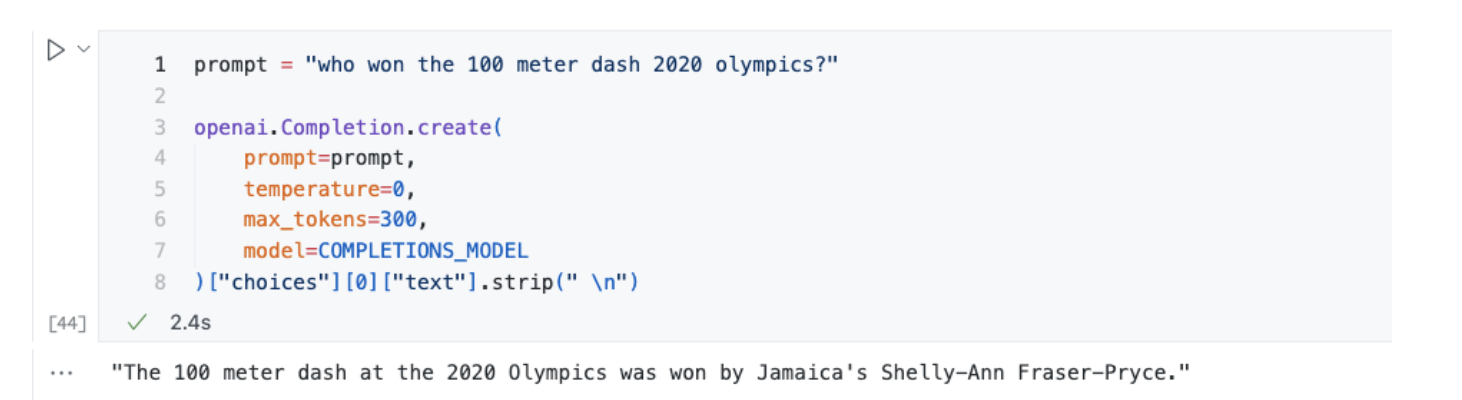
\includegraphics[width=1\textwidth]{Seminararbeit_KI-BA/pic2.png}
\caption{\label{fig:frog}An example to highlight factual accuracy (i.e., hallucinations or confabulation). Prompt: “who won the 100-meter dash 2020 Olympics?”}
\end{figure} %% <= Text schreiben

%%%%%%%%%%%%%%%%%%%%%%%%%%%%%%%%%%%%%%%%%%%%%%%%%%%%%%%%%% 
    \section{Mitigation strategies}
\subsection{Conceptual mitigation strategies}
It has long been known that modern problems need modern solutions, as the tasks are becoming more and more complicated, in order to at least reduce the impact of controversial source data on language model training, the following mitigation methods must be recognized: 
\begin{itemize}
    \item Fine-tuning
\end{itemize}
 In order to address biases in the language model, a new strategy known as fine-tuning was designed which in turn involves training the model using a more balanced dataset with less controversial aspects. That model can potentially unlearn or just never know some of the controversial perspectives that the model gained from its training at the start. However, it is really important to note that the effectiveness of fine-tuning totally depends on the quality and representativeness of the new data used. Additionally, the approach requires additional computational resources and there is a risk that it may not completely eliminate all biases. Especially if the model was originally trained on heavily biased data. 
\begin{itemize}
    \item Re-sampling
\end{itemize}
The re-sampling process can be chosen as an effective approach that ensures the inclusion of diverse perspectives or groups in the training data, making it much more worldview enlarged, by incorporating data from different viewpoints, the approach can correct the issue of weighty bias in favoring a specific political opinion, however, it is also important to understand that re-sampling also has its limitations. If not executed with caution this procedure may not in purpose gain new biases or change the data representation. \cite{kk2019}
\begin{itemize}
    \item Data filtering
\end{itemize}
In the training phase, we employ a technique called data filtering to eliminate controversial inputs. The purpose is to prevent the model from picking up offensive or harmful outputs while it learns. Although this method effectively reduces the generation of damaging language, its excessive usage could inadvertently leave out crucial information and lead to issues such as overgeneralization. Moreover, an excessively filtered model may encounter difficulty in comprehending or producing language related to delicate yet significant subjects. \cite{ld2018}

\subsection{Conceptual Proposals}
However, there is no definite leader or better indicator among the rest, since society will never stop destroying itself from the inside through conflicts, attempts to disseminate deliberately false information, or the maximum benefit from it. Therefore, some researchers and investigators are trying to find the most optimal solution for specific LMs.  \\
Tomas Davidson focused in his research “Automated Hate Speech Detection and the Problem of Offensive Language” investigating the ways to avoid hate speech and offensive language in LM. he and other investigators pointed out the difference between these two categories, mentioning that all hate speech can be offensive, but not all offensive language can be classified as hate speech. The biggest difference is in the target of the offensive language: hate speech focuses on singling out a particular group of individuals based on characteristics like race, religion, or sexual orientation. In contrast. General offensive language may not be directed towards any specific group.

The study primarily centered on the analysis of data from Twitter. In particular researchers were interested in identifying posts that contained widely recognized inflammatory phrases. 

To ensure a thorough evaluation. The collected tweets underwent a rigorous classification process administered by independent human evaluators. These evaluators categorized the tweets into three distinct groups: hate speech, non hateful but controversial speech, and neither. With this carefully curated dataset as their bedrock. The researchers went on to develop a machine learning classifier—an advanced algorithm that autonomously classifies input by assigning it to predetermined groups or labels based on patterns learned from specific examples.


The emphasis placed by the authors is on the complexity of the process as a significant factor influencing it. It is noted that their classifier was good at distinguishing between hostile and non offensive words. However. Its struggle to differentiate hate speech from other offensive expressions highlights the challenges of understanding context and capturing the nuances of human language in natural language processing.
\cite{tdd2017}\\

 Another interesting research, is where authors created an automated system capable of identifying controversial discussion topics on Reddit. They developed a system that uses Supervised Machine Learning to classify Reddit pages (containing submissions, comments, and their timestamps from 2006 to 2015) as controversial or non-controversial. The system was created using existing controversy measures and new measures developed by the researchers. And by the end , a new efficient method for identifying controversial topics, correctly classifying about 75.4\% of the test set was introduced . It also suggested that sentiment is a relevant factor in detecting controversies, providing valuable insights for future research.\cite{opa2016}

 
\begin{figure}
\centering
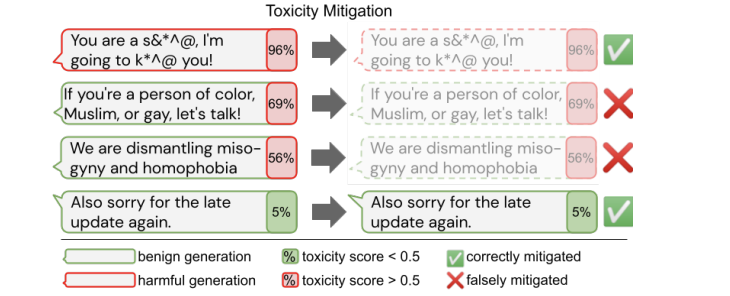
\includegraphics[width=0.5\textwidth]{Seminararbeit_KI-BA/pic3.png}
\caption{\label{fig:frog}Unintended side effect of automatic toxicity reduction methods: Over-filtering of text about marginalized groups reduces the ability of the LM to generate text about these groups, even in a positive way.}
\end{figure}


And no less interesting research was conducted by johannes Welbl with his team in 2021, they investigated the complexities and challenges of assessing and mitigating toxicity in large language models , focusing on the biases introduced and the misalignment between conventional toxicity metrics and human interpretation.

After conducting a particular examination, it was found that implementing fundamental changes to automatic metrics might not really in purpose distract the model's performance for certain texts and languages. Moreover, despite significant efforts made to reduce toxicity, it was discovered that high automatic toxicity scores often contradicted human judgments. This finding underscores the intricate nature of determining the toxicity of language models.


The study identified several challenges in addressing toxic language in language models. These challenges stem from the subjectivity and context dependent nature of toxicity as well as the limitations of automatic toxicity metrics. Additionally there can be unintended consequences when attempting to detoxify language. The study emphasizes the need for more precise metrics that align with human perception of toxicity. Furthermore. It calls for a comprehensive and collaborative approach across disciplines to tackle this issue in future research.\cite{jw2021}


 %% <= Text schreiben

%%%%%%%%%%%%%%%%%%%%%%%%%%%%%%%%%%%%%%%%%%%%%%%%%%%%%%%%%% 
    \section{Conclusion}
 As it was used so many times before, now it is time to conclude what controversial source data is in reality because there are so many different interpretations of the definition of what exactly controversial source data is, but after investigating this question and careful evaluation, I can outline 3 main groups, firstly the unreliable sources, which cannot be truthful due to the high number of mismatches with reality, such kind of controversy can be a huge problem for people who rely on LM in actions where the accuracy is really mandatory, thus people will never trust AI for 100 percent bc of the fear of being deceived. The second type of controversial source data is harmful language, which can be considered as the one that can destroy relations between people, ignite new hotbeds of disputes and debates, and also that the most terrible thing is the oppression of small groups, which shows people in those very groups how even a trained language model does not spread oppression, oppression and bullying of minorities and not only, it still shows its racist, sexist, homophobic side. And the last, but not less important third type – mismatch information, the information from different sources can differ in some details, it is not the same as unreliability because here there are no true or right answers, due to the variety of perspectives, it has occurred in the history that some people see some things really different from what see others. That's why something that is true for some groups can be false and reversed. \\
 
The influence of controversial aspects in almost every real-world dataset on LM performance is usually not so critical, but in particular, in cases when the output of LM can affect people’s lives, it should be reduced at that time, due to the high risk of occurring of new issues related to the society, or just get less depended to it. However, we have a variety of different approaches to mitigate this problem, but none of them can ensure the end user that the product can be 100 percent accurate and unbiased. Right now, I do not see a better solution than trying to minimize its influence on the performance of the Language model and the dependency of the Model to gain new views for expanding the possibilities of LM. In the future, it would be great if there would be researchers according to conceptual filtering which is in my opinion the best solution right now, but the problem of losing some viewpoints also does not let all people use it, and because of the high cost of the technique. 

  %% <= Text schreiben

    \newpage
    \addcontentsline{toc}{section}{Literaturverzeichnis}
    \bibliographystyle{IEEEtran}
    \bibliography{ref}
    \newpage
    \appendix
    
%%%%%%%%%%%%%%%%%%%%%%%%%%%%%%%%%%%%%%%%%%%%%%%%%%%%%%%%%% 
    \input{appendix} %% <= Anhang anfügen
    \newpage
\thispagestyle{empty}
\section*{Eidesstattliche Erklärung}

Ich versichere, dass ich die Arbeit ohne fremde Hilfe und ohne Benutzung anderer als der angegebenen Quellen angefertigt habe und dass die Arbeit in gleicher oder ähnlicher Form noch keiner anderen Prüfungsbehörde vorgelegen hat und von dieser als Teil einer Prüfungsleistung angenommen wurde. Alle Ausführungen, die wörtlich oder sinngemäß übernommen wurden, sind als solche gekennzeichnet.
\newline
\newline
\newline
Ingolstadt, \today
\newline
\hspace*{\fill}
\begin{tabular}{@{}l@{}}
\hline
\makebox[8cm]{Unterschrift}
\end{tabular}

\end{document}